\documentclass{article}
\usepackage[utf8]{inputenc}
\usepackage{graphicx}
\usepackage{wrapfig}
\usepackage{caption}
\usepackage{lipsum} 


\title{Assingment 2}
\author{}
\date{}

\begin{document}

\maketitle

1. \begin{wrapfigure}{r}{0.4\textwidth}
    \centering
    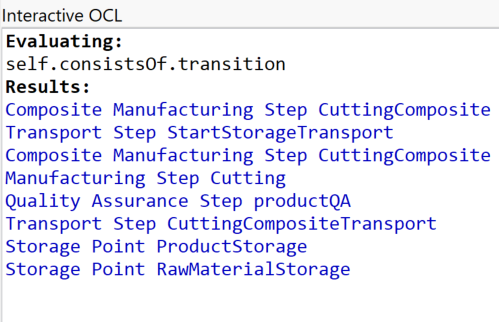
\includegraphics[width=0.38\textwidth]{images/Pasted image 20250518183913.png}
    \caption{OCLConsole}
    \label{fig:metamodel}
\end{wrapfigure}

In the given metamodel, the ManufacturingSystem EClass contains one or more ManufacturingSystemElement instances, with this containment relationship named consistsOf. Additionally, ManufacturingSystemElement instances can have transitions to other ManufacturingSystemElement instances. As a result, invoking self.consistsOf.transition returns all transitions among the ManufacturingSystemElements contained within a FurnitureSystem. Upon manual inspection of the model, it is observed that the ManufacturingSystemElements include StoragePoint (such as ProductStorage and RawMaterialStorage) and various types of Step elements (ManufacturingStep, TransportStep, QualityAssuranceStep, and CompositeManufacturingStep). When self.consistsOf.transition() is evaluated, it should return all transitions between these elements. The model reveals the following transitions: from RawMaterialStorage to both CuttingComposite and StartStorageTransport, from StartStorageTransport to CuttingComposite and Cutting, from CuttingComposite to ProductQA, from ProductQA to CuttingCompositeTransport, from CuttingCompositeTransport to ProductStorage, and from ProductStorage back to RawMaterialStorage. The OCLConsole returns all these transitions (see Figure~\ref{fig:metamodel}).



2. \begin{wrapfigure}{r}{0.4\textwidth}
    \centering
    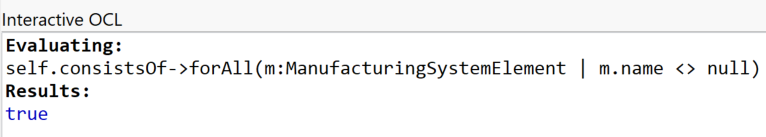
\includegraphics[width=0.38\textwidth]{images/Screenshot 2025-05-18 191855.png}
    \caption{OCLConsole 2.Expression}
    \label{fig:ex2}
\end{wrapfigure}


The second expression is an expression used to check that all ManufacturingSystemElement instances within the FurnitureSystem have a non-null name. In other words, this expression returns true if every ManufacturingSystemElement inside the FurnitureSystem has a name. If even one of them does not have a name, it returns false. During manual inspection, it was observed that each ManufacturingSystemElement had a name, so the expression correctly returned true (see Figure~\ref{fig:ex2}).

\newpage

3. \begin{wrapfigure}{r}{0.4\textwidth}
    \centering
    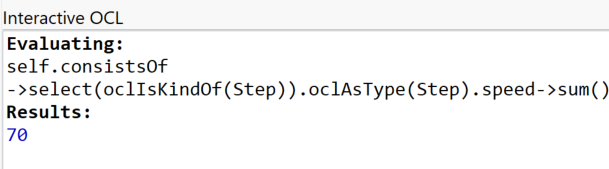
\includegraphics[width=0.38\textwidth]{images/ex3.png}
    \caption{OCLConsole 3.Expression}
    \label{fig:ex3}
\end{wrapfigure}
All classes of type Step have a speed attribute. The third expression is expected to sum the speed values of all instances of type Step within the FurnitureSystem and return the result. When calculated manually, this expression should yield (20 + 20 + 10 + 20) = 70. Executing this expression in the OCL Console also returns 70 as the output (see Figure~\ref{fig:ex3}).


4. \begin{wrapfigure}{r}{0.4\textwidth}
    \centering
    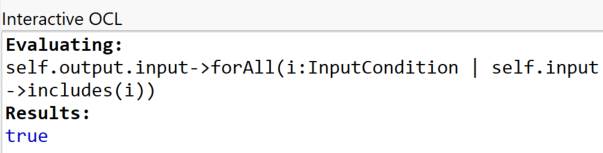
\includegraphics[width=0.38\textwidth]{images/ex4.png}
    \caption{OCLConsole 4.Expression}
    \label{fig:ex4}
\end{wrapfigure}

The Step class has references to the InputCondition and OutputDecision EClasses, representing its inputs and outputs, respectively. The fourth expression operates in the context of CuttingCompositeTransport and checks whether all the required inputs for the next step are available.
Within CuttingCompositeTransport, there are two types of OutputDecision, each expecting final\_wood and final\_metal as inputs, respectively.
Since both of these inputs are present within the CuttingCompositeTransport step, the fourth expression should evaluate to true (see Figure~\ref{fig:ex4}).


5. MISSING

6. MISSING
\end{document}

